The showcase uses the architecture as a base and adds features referencing the research topic. The simulation image of the showcase is built upon the simulation image of the architecture, it adds an OctoMap plugin for RViz and a \acs{qrcode} detector for each simulated \acs{uav}. The \acs{slam} image is also built from the simulation of the architecture because it needs a \acs{gui} to show the created point cloud and other information. The \acs{slam} image has \acs{rtabmap} and all of its dependencies installed. Both the planner and the vision images are built from the \acs{ros} Melodic image. The planner image has Octomap for Python installed and the vision image installs a transformation to calculate the yaw from a quaternion.

\begin{figure}[!h]
  \centering
  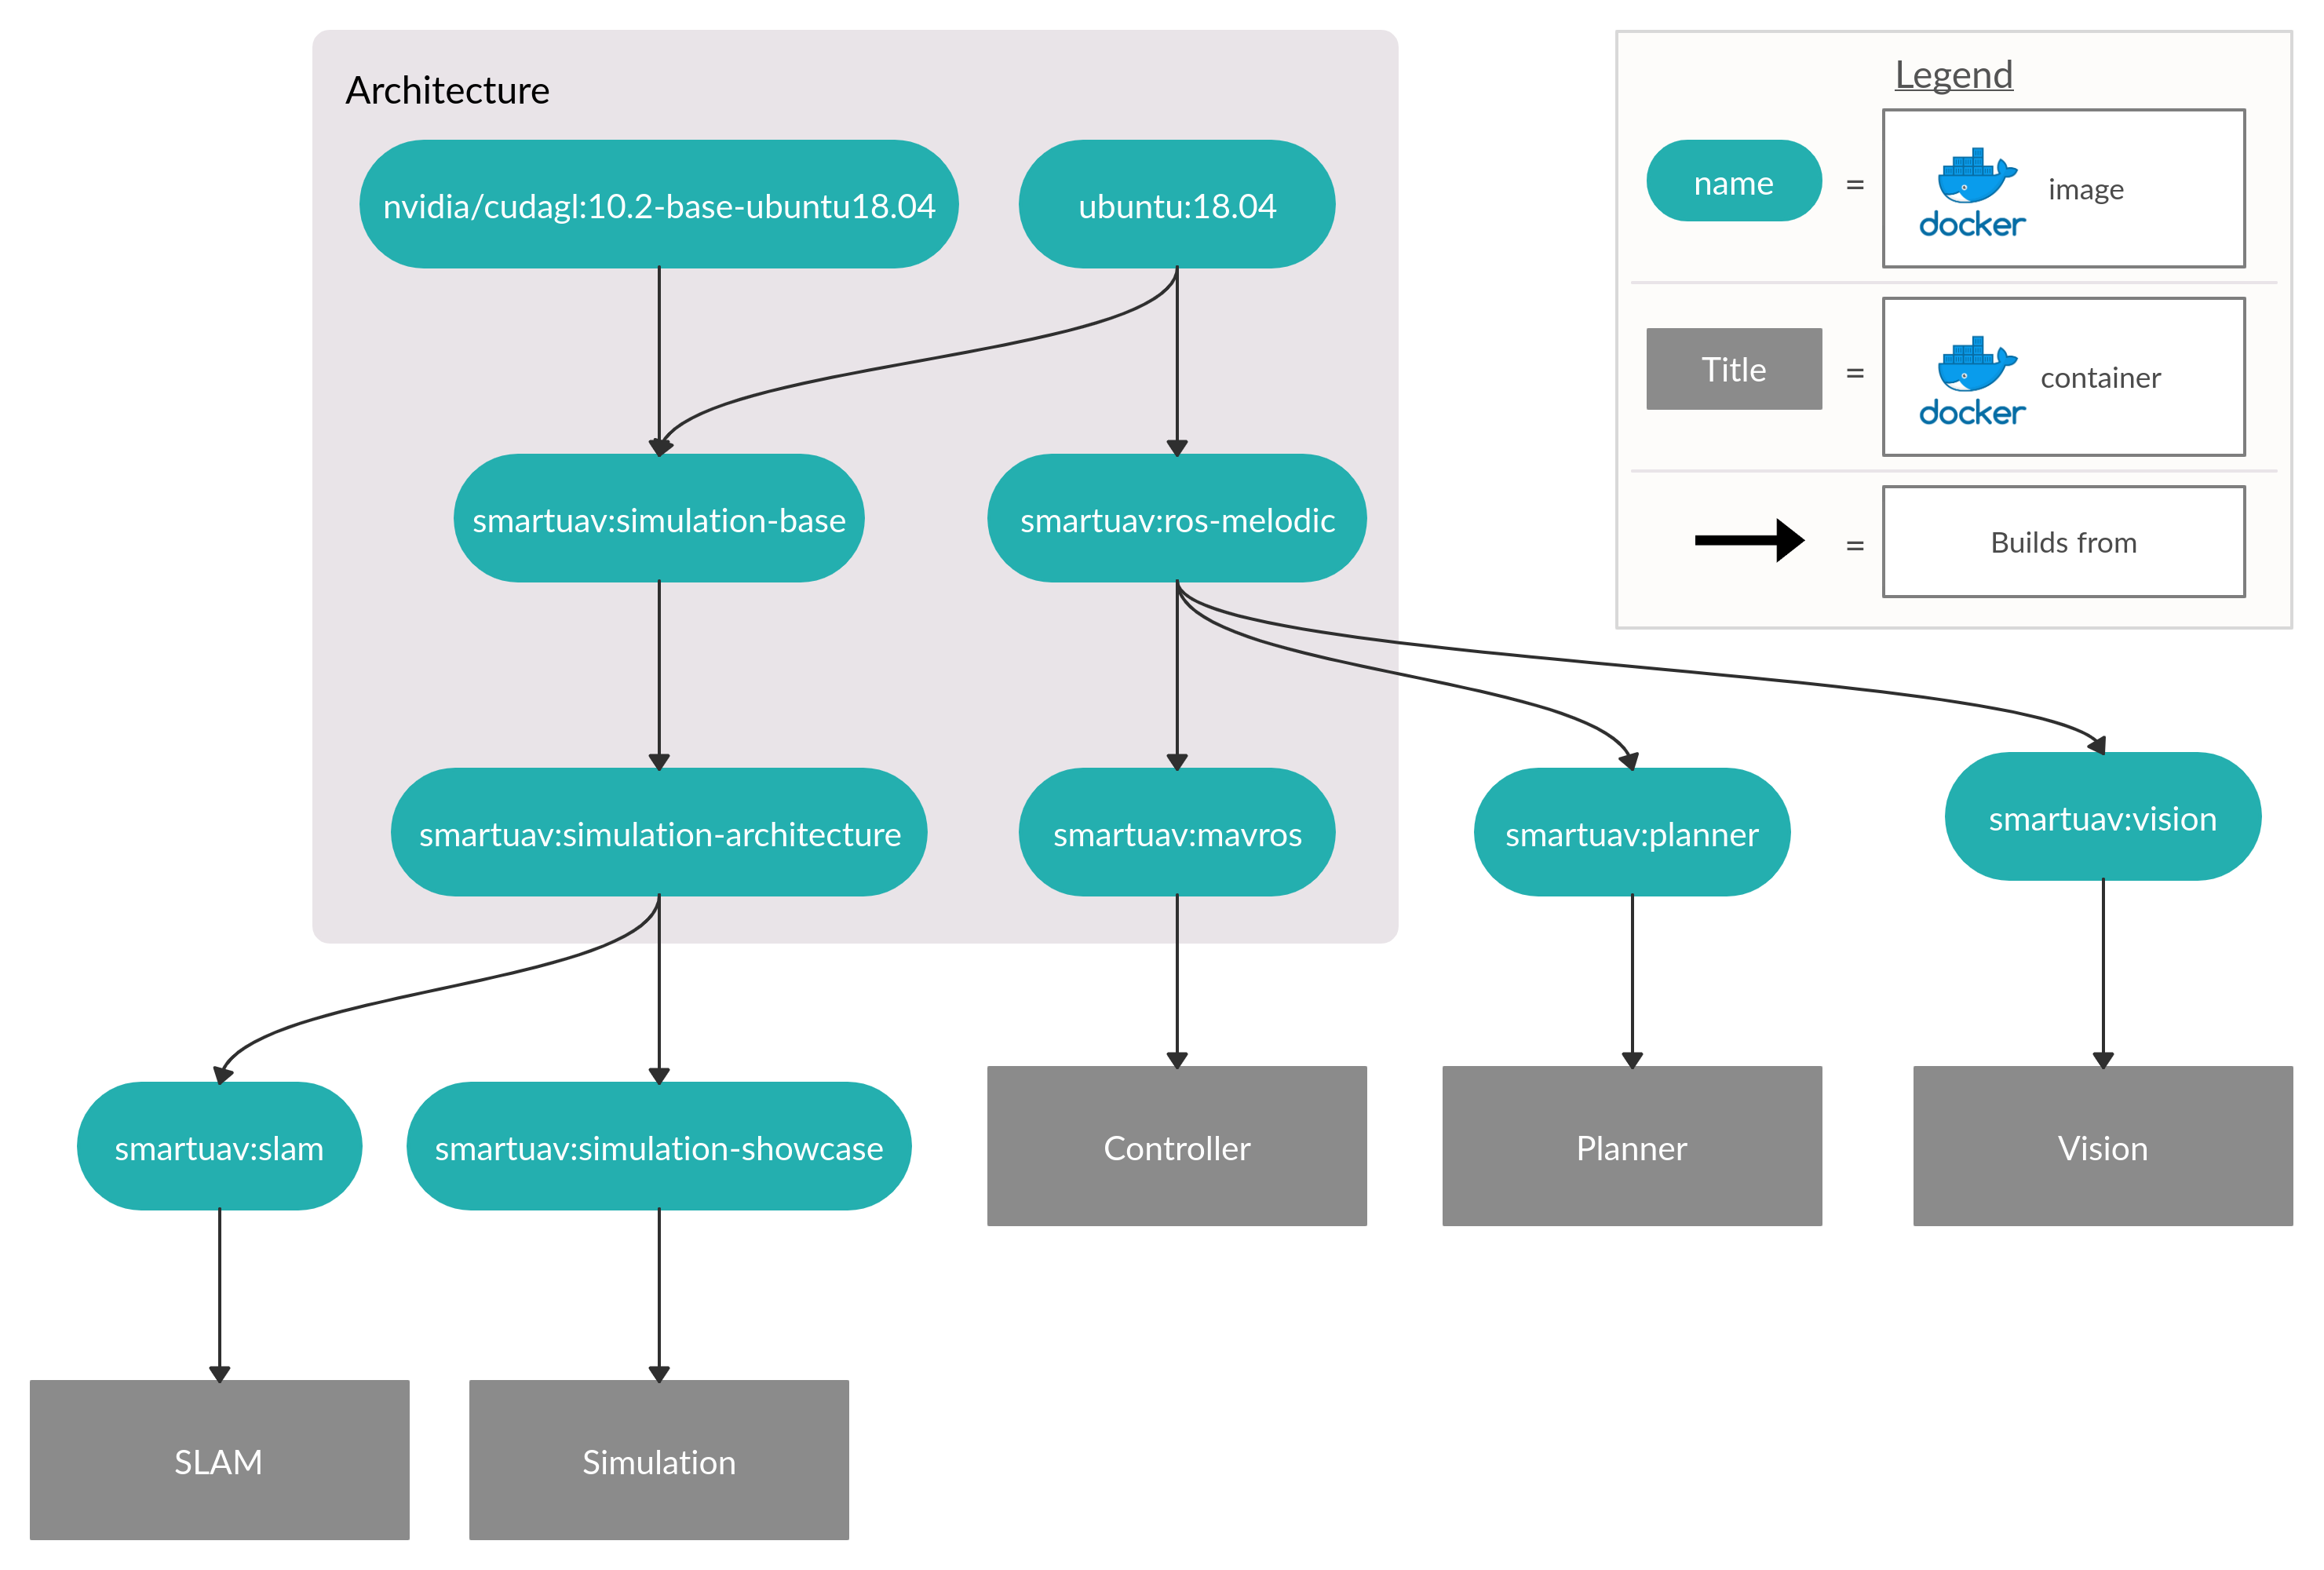
\includegraphics[width=\linewidth]{images/showcase_images.png}
  \caption{Docker images showcase}
\end{figure}

\clearpage

The showcase is used to conduct research, visualize this research, and show the capabilities of the architecture. Figure~\ref{fig:showcase_containers} visualizes which containers are run in the showcase and how there are connected.

\begin{figure}[!h]
  \centering
  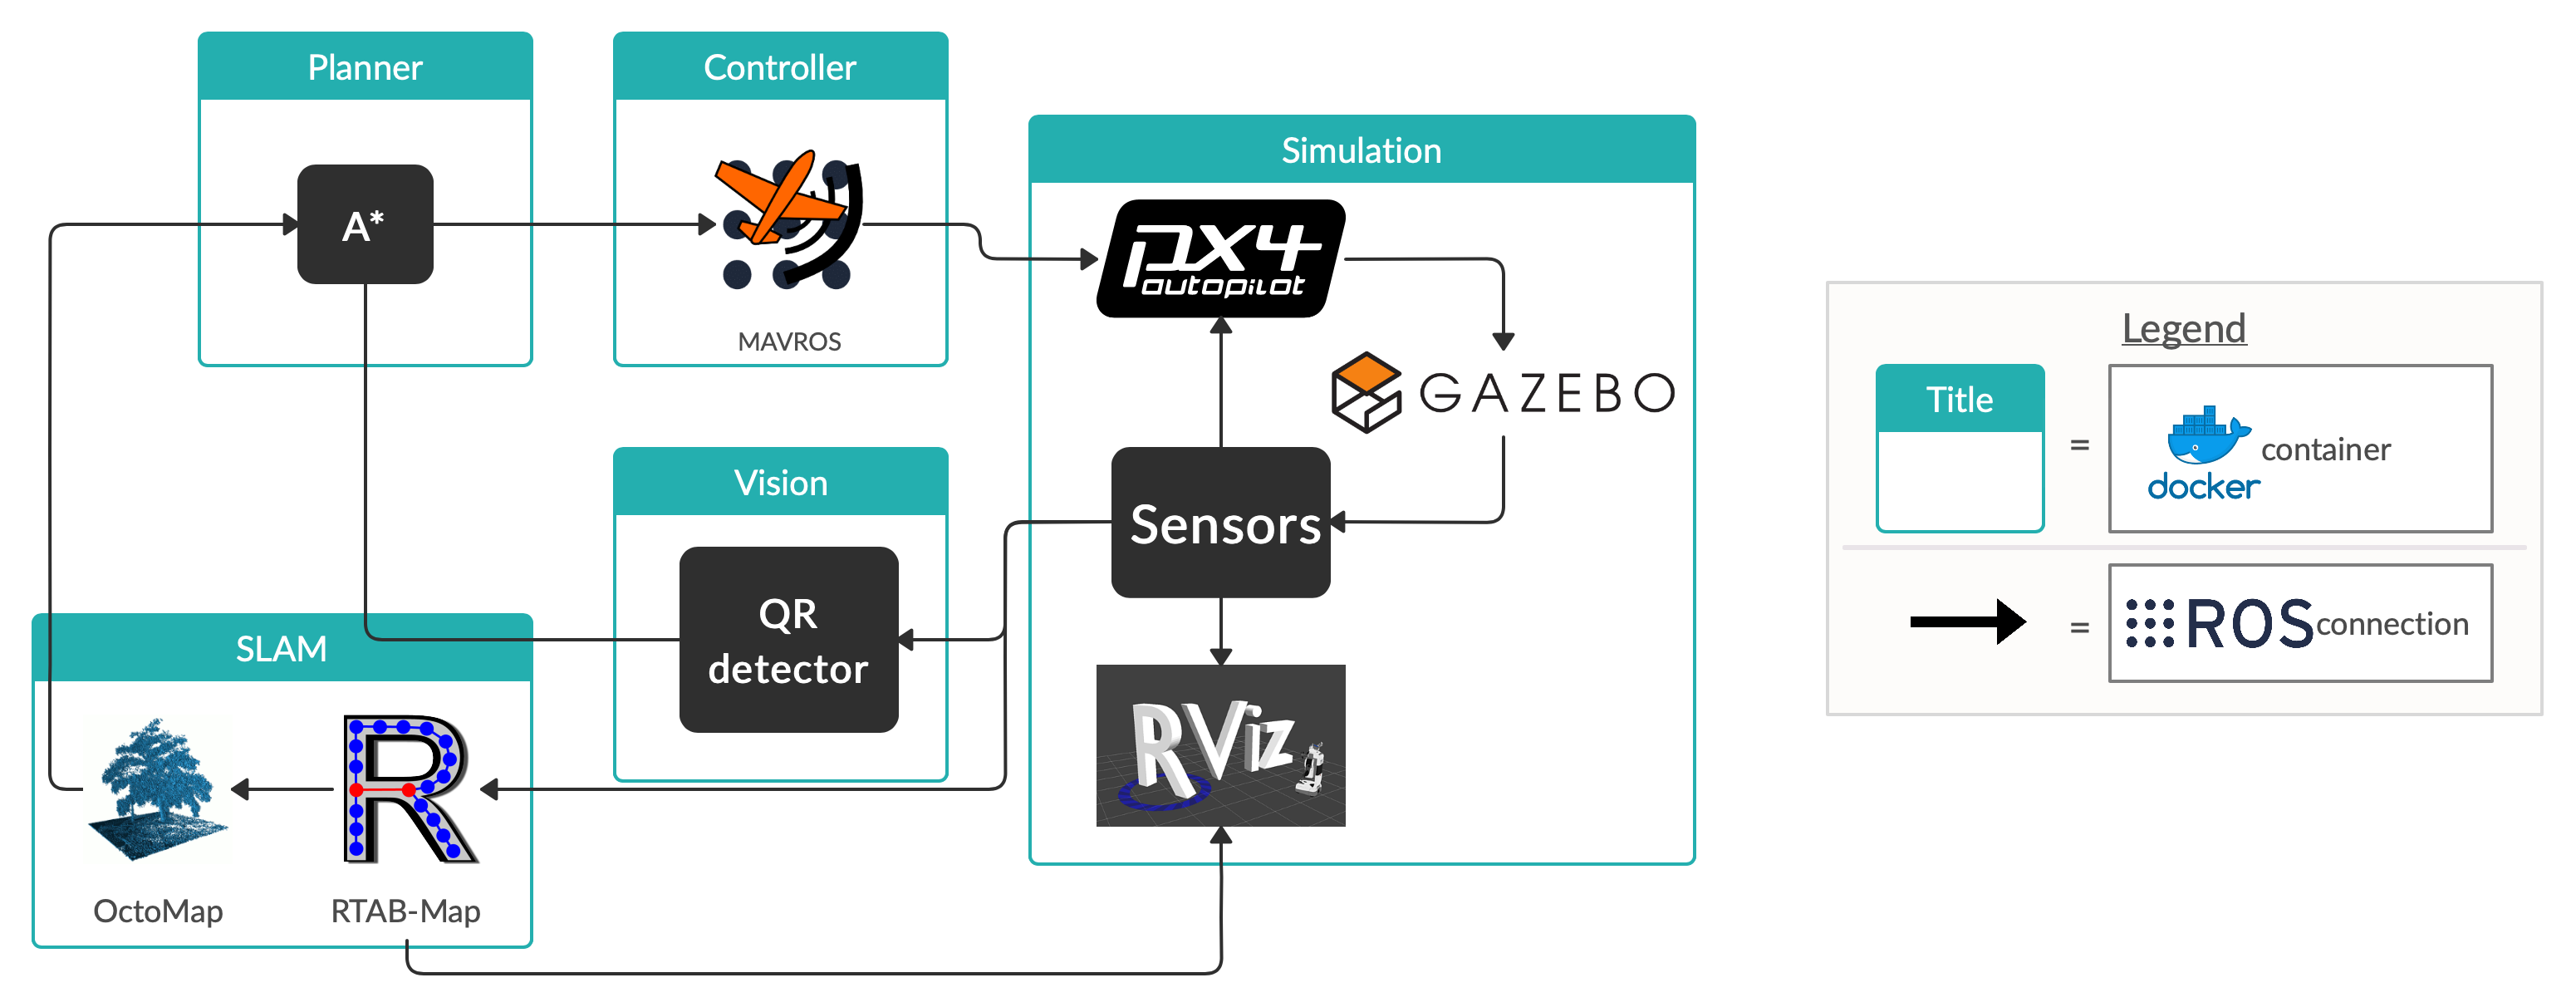
\includegraphics[width=\linewidth]{images/showcase_containers.png}
  \caption{Docker containers showcase}
  \label{fig:showcase_containers}
\end{figure}